% Options for packages loaded elsewhere
\PassOptionsToPackage{unicode}{hyperref}
\PassOptionsToPackage{hyphens}{url}
%
\documentclass[
  ignorenonframetext,
]{beamer}
\usepackage{pgfpages}
\setbeamertemplate{caption}[numbered]
\setbeamertemplate{caption label separator}{: }
\setbeamercolor{caption name}{fg=normal text.fg}
\beamertemplatenavigationsymbolsempty
% Prevent slide breaks in the middle of a paragraph
\widowpenalties 1 10000
\raggedbottom
\setbeamertemplate{part page}{
  \centering
  \begin{beamercolorbox}[sep=16pt,center]{part title}
    \usebeamerfont{part title}\insertpart\par
  \end{beamercolorbox}
}
\setbeamertemplate{section page}{
  \centering
  \begin{beamercolorbox}[sep=12pt,center]{part title}
    \usebeamerfont{section title}\insertsection\par
  \end{beamercolorbox}
}
\setbeamertemplate{subsection page}{
  \centering
  \begin{beamercolorbox}[sep=8pt,center]{part title}
    \usebeamerfont{subsection title}\insertsubsection\par
  \end{beamercolorbox}
}
\AtBeginPart{
  \frame{\partpage}
}
\AtBeginSection{
  \ifbibliography
  \else
    \frame{\sectionpage}
  \fi
}
\AtBeginSubsection{
  \frame{\subsectionpage}
}
\usepackage{amsmath,amssymb}
\usepackage{iftex}
\ifPDFTeX
  \usepackage[T1]{fontenc}
  \usepackage[utf8]{inputenc}
  \usepackage{textcomp} % provide euro and other symbols
\else % if luatex or xetex
  \usepackage{unicode-math} % this also loads fontspec
  \defaultfontfeatures{Scale=MatchLowercase}
  \defaultfontfeatures[\rmfamily]{Ligatures=TeX,Scale=1}
\fi
\usepackage{lmodern}
\ifPDFTeX\else
  % xetex/luatex font selection
\fi
% Use upquote if available, for straight quotes in verbatim environments
\IfFileExists{upquote.sty}{\usepackage{upquote}}{}
\IfFileExists{microtype.sty}{% use microtype if available
  \usepackage[]{microtype}
  \UseMicrotypeSet[protrusion]{basicmath} % disable protrusion for tt fonts
}{}
\makeatletter
\@ifundefined{KOMAClassName}{% if non-KOMA class
  \IfFileExists{parskip.sty}{%
    \usepackage{parskip}
  }{% else
    \setlength{\parindent}{0pt}
    \setlength{\parskip}{6pt plus 2pt minus 1pt}}
}{% if KOMA class
  \KOMAoptions{parskip=half}}
\makeatother
\usepackage{xcolor}
\newif\ifbibliography
\usepackage{longtable,booktabs,array}
\usepackage{calc} % for calculating minipage widths
\usepackage{caption}
% Make caption package work with longtable
\makeatletter
\def\fnum@table{\tablename~\thetable}
\makeatother
\usepackage{graphicx}
\makeatletter
\newsavebox\pandoc@box
\newcommand*\pandocbounded[1]{% scales image to fit in text height/width
  \sbox\pandoc@box{#1}%
  \Gscale@div\@tempa{\textheight}{\dimexpr\ht\pandoc@box+\dp\pandoc@box\relax}%
  \Gscale@div\@tempb{\linewidth}{\wd\pandoc@box}%
  \ifdim\@tempb\p@<\@tempa\p@\let\@tempa\@tempb\fi% select the smaller of both
  \ifdim\@tempa\p@<\p@\scalebox{\@tempa}{\usebox\pandoc@box}%
  \else\usebox{\pandoc@box}%
  \fi%
}
% Set default figure placement to htbp
\def\fps@figure{htbp}
\makeatother
\setlength{\emergencystretch}{3em} % prevent overfull lines
\providecommand{\tightlist}{%
  \setlength{\itemsep}{0pt}\setlength{\parskip}{0pt}}
\setcounter{secnumdepth}{-\maxdimen} % remove section numbering
\usepackage{bookmark}
\IfFileExists{xurl.sty}{\usepackage{xurl}}{} % add URL line breaks if available
\urlstyle{same}
\hypersetup{
  hidelinks,
  pdfcreator={LaTeX via pandoc}}

\author{}
\date{\vspace{-2.5em}}

\begin{document}

\begin{frame}

Session 1 - Policy Evaluation
\end{frame}

\begin{frame}{Introduction to policy evaluation}
\phantomsection\label{introduction-to-policy-evaluation}
\textbf{Lecturer:}\\
Andreas Steinmayr\\
University of Innsbruck\\
Fall 2023

\emph{Core reading: Gertler, chapters 1 and 2}
\end{frame}

\begin{frame}{Mean annual earnings of full-time workers in Austria 2017}
\phantomsection\label{mean-annual-earnings-of-full-time-workers-in-austria-2017}
\pandocbounded{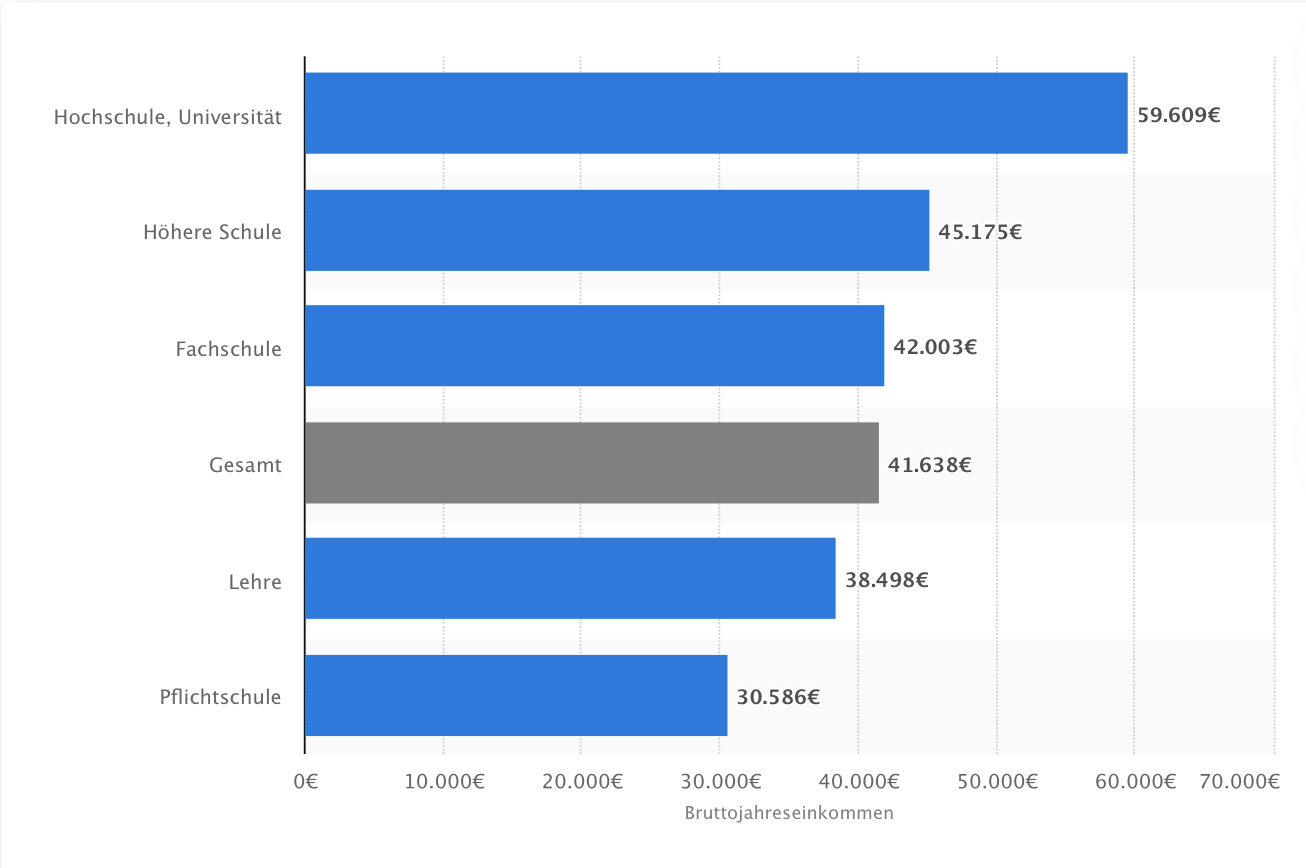
\includegraphics[keepaspectratio]{figures/earnings_austria_2017}}\\
\emph{Source: Statistik Austria, Statista 2022}
\end{frame}

\begin{frame}{Purpose of this course}
\phantomsection\label{purpose-of-this-course}
\begin{itemize}
\tightlist
\item
  \textbf{Understand program evaluation as a \emph{consumer}}

  \begin{itemize}
  \tightlist
  \item
    Synthesize and understand evaluation results\\
  \item
    Evaluate the quality of policy evaluations or choose between
    evaluation proposals\\
  \item
    Make evidence-based decisions\\
  \end{itemize}
\item
  \textbf{Provide skills to design and implement program evaluations}

  \begin{itemize}
  \tightlist
  \item
    Many economists work on evaluations, not only in academia
  \end{itemize}
\end{itemize}
\end{frame}

\begin{frame}{Why do we evaluate programs?}
\phantomsection\label{why-do-we-evaluate-programs}
\begin{itemize}
\tightlist
\item
  \textbf{Policy} and \textbf{program} will be used as synonyms\\
\item
  Lots of money is spent every year to try to change things:

  \begin{itemize}
  \tightlist
  \item
    Government-provided job training programs\\
  \item
    Sugar-tax to reduce obesity\\
  \item
    Subsidies to increase R\&D investment in firms\\
  \item
    Incentive schemes to increase worker productivity\\
  \end{itemize}
\item
  We want to know:

  \begin{itemize}
  \tightlist
  \item
    What difference have these programs made?\\
  \item
    What outcomes have been affected? By how much and for whom?
  \end{itemize}
\end{itemize}
\end{frame}

\begin{frame}{Broader agenda: Evidence-based policy making}
\phantomsection\label{broader-agenda-evidence-based-policy-making}
\begin{itemize}
\tightlist
\item
  Policy decisions informed by rigorously established evidence

  \begin{itemize}
  \tightlist
  \item
    In reality often: \emph{Policy-based evidence making}\\
  \end{itemize}
\item
  Based on the idea of evidence-based medicine\\
\item
  Goal: Inform allocation of resources, guide policy decisions, enhance
  accountability\\
\item
  Build general knowledge about the effectiveness of policies
\end{itemize}
\end{frame}

\begin{frame}{Which policies should we evaluate?}
\phantomsection\label{which-policies-should-we-evaluate}
\begin{itemize}
\tightlist
\item
  Evaluations are costly, especially data collection\\
\item
  What are the stakes of this policy?

  \begin{itemize}
  \tightlist
  \item
    Budget\\
  \item
    Size of target population\\
  \item
    \emph{Potential} effect sizes\\
  \end{itemize}
\item
  Evaluate if the policy is:

  \begin{itemize}
  \tightlist
  \item
    Innovative: new and promising\\
  \item
    Replicable: can be scaled up or applied in a different setting\\
  \item
    Strategically relevant: flagship initiative, requires substantial
    resources, could have large (side) effects or generate substantial
    savings\\
  \item
    Untested: Little is known about the effectiveness of this type of
    policy\\
  \item
    Influential: Results will be used to inform key policy decisions
  \end{itemize}
\end{itemize}
\end{frame}

\begin{frame}{Common errors}
\phantomsection\label{common-errors}
\begin{itemize}
\tightlist
\item
  People without knowledge in program evaluation tend to confuse:

  \begin{itemize}
  \tightlist
  \item
    Monitoring and evaluation\\
  \item
    Correlation and impacts\\
  \end{itemize}
\item
  Examples:

  \begin{itemize}
  \tightlist
  \item
    ``The program was successful: 72\% of participants find a job after
    job training''\\
  \item
    ``I feel better today because I took Globuli yesterday''\\
  \item
    ``She has a high income because she studied economics''\\
  \item
    ``Aztecs: Without human sacrifices of children, rain would not come,
    and crops would not flourish''\\
  \end{itemize}
\item
  This can be extremely misleading
\end{itemize}
\end{frame}

\begin{frame}{Simpson's (1951) paradox}
\phantomsection\label{simpsons-1951-paradox}
\begin{itemize}
\tightlist
\item
  Event C increases the probability of E in the population, whereas it
  decreases the probability of E in all sub-populations\\
\item
  Example: Taking a particular pill is helpful for the population but
  harmful for men and women
\end{itemize}

\begin{longtable}[]{@{}lllll@{}}
\toprule\noalign{}
Combined & Recovery (E) & Not E & Sum & Recovery Rate \\
\midrule\noalign{}
\endhead
Drug (C) & 20 & 20 & 40 & 50\% \\
No drug (not C) & 16 & 24 & 40 & 40\% \\
\bottomrule\noalign{}
\end{longtable}
\end{frame}

\begin{frame}{What is impact evaluation?}
\phantomsection\label{what-is-impact-evaluation}
\begin{itemize}
\tightlist
\item
  \textbf{Monitoring} tracks what is happening with a program, looks at
  the program implementation

  \begin{itemize}
  \tightlist
  \item
    Is the money indeed spent the way it was supposed to be?\\
  \end{itemize}
\item
  \textbf{Impact evaluations} seek to answer a cause-and-effect question

  \begin{itemize}
  \tightlist
  \item
    Which changes are directly attributable to a program?\\
  \item
    What is the effect of obtaining a university degree on earnings?
  \end{itemize}
\end{itemize}
\end{frame}

\begin{frame}{Prospective versus retrospective evaluation}
\phantomsection\label{prospective-versus-retrospective-evaluation}
\begin{itemize}
\tightlist
\item
  \textbf{Prospective evaluation}

  \begin{itemize}
  \tightlist
  \item
    Set up at the same time as policy\\
  \item
    Built into policy implementation/roll-out\\
  \end{itemize}
\item
  \textbf{Retrospective evaluation}

  \begin{itemize}
  \tightlist
  \item
    Policy evaluation after implementation\\
  \end{itemize}
\item
  PE is more likely to produce credible evaluation results

  \begin{itemize}
  \tightlist
  \item
    (Baseline) data collection on treated and controls\\
  \item
    Creates focus on policy objectives\\
  \item
    Easier to construct credible counterfactual
  \end{itemize}
\end{itemize}
\end{frame}

\begin{frame}{Efficacy studies and effectiveness studies}
\phantomsection\label{efficacy-studies-and-effectiveness-studies}
\begin{itemize}
\tightlist
\item
  \textbf{Efficacy studies}

  \begin{itemize}
  \tightlist
  \item
    Carried out in a specific setting under closely controlled
    conditions\\
  \item
    Small-scale pilot/proof of concept\\
  \end{itemize}
\item
  \textbf{Effectiveness studies}

  \begin{itemize}
  \tightlist
  \item
    Interventions that take place in normal circumstances, using regular
    implementation channels\\
  \item
    Aim to produce findings that can be generalized to a large
    population
  \end{itemize}
\end{itemize}
\end{frame}

\begin{frame}{Internal versus external validity}
\phantomsection\label{internal-versus-external-validity}
\begin{itemize}
\tightlist
\item
  \textbf{Internal validity}

  \begin{itemize}
  \tightlist
  \item
    Evaluation identifies causal effect of program in a given setting\\
  \item
    Varying degrees of credibility (RCT: Gold Standard)\\
  \end{itemize}
\item
  \textbf{External validity}

  \begin{itemize}
  \tightlist
  \item
    Generalizability of causal effect to other situations\\
  \item
    Informative for a larger or different population, different time
  \end{itemize}
\end{itemize}
\end{frame}

\begin{frame}{Cost-benefit and cost-effectiveness analysis}
\phantomsection\label{cost-benefit-and-cost-effectiveness-analysis}
\begin{itemize}
\tightlist
\item
  \textbf{Cost-benefit analysis}

  \begin{itemize}
  \tightlist
  \item
    Estimates the total expected benefits of a program, compared to its
    total expected costs.\\
  \item
    Seeks to quantify all of the costs and benefits of a program in
    monetary terms and assesses whether benefits outweigh costs.\\
  \end{itemize}
\item
  \textbf{Cost-effectiveness analysis}

  \begin{itemize}
  \tightlist
  \item
    Compares the relative cost of two or more programs or program
    alternatives in reaching a common outcome\\
    Impact evaluation estimates the benefit side, and cost analysis
    provides the cost information! We focus on \textbf{impact
    evaluation}.
  \end{itemize}
\end{itemize}
\end{frame}

\begin{frame}{Preparing for an evaluation}
\phantomsection\label{preparing-for-an-evaluation}
\begin{itemize}
\tightlist
\item
  Specify the evaluation question\\
\item
  Construct a theory of change\\
\item
  Develop a results chain\\
\item
  Select indicators to assess performance
\end{itemize}
\end{frame}

\begin{frame}{Evaluation question}
\phantomsection\label{evaluation-question}
\begin{itemize}
\tightlist
\item
  First step: Formulate a clear study question

  \begin{itemize}
  \tightlist
  \item
    What is the impact of the policy on an outcome of interest?\\
  \item
    Which changes are directly attributable to a program?\\
  \end{itemize}
\item
  Needs to be framed as a \textbf{well-defined, testable hypothesis}
\end{itemize}
\end{frame}

\begin{frame}{Are these good evaluation questions?}
\phantomsection\label{are-these-good-evaluation-questions}
\begin{itemize}
\tightlist
\item
  What is the effect of studying economics on later earnings?\\
\item
  What is the effect of being a woman on the likelihood of becoming a
  politician?\\
\item
  What is the effect of reducing the speed limit on highways from 130 to
  100 km/h on the number of traffic deaths?
\end{itemize}
\end{frame}

\begin{frame}{Theory of change}
\phantomsection\label{theory-of-change}
\begin{itemize}
\tightlist
\item
  Describe the causal pathway (sequence of events from policy to final
  outcomes)\\
\item
  Formulate necessary assumptions and enabling conditions\\
\item
  Include all stakeholders\\
\item
  Consult existing literature
\end{itemize}
\end{frame}

\begin{frame}{Results chain}
\phantomsection\label{results-chain}
\begin{figure}
\centering
\pandocbounded{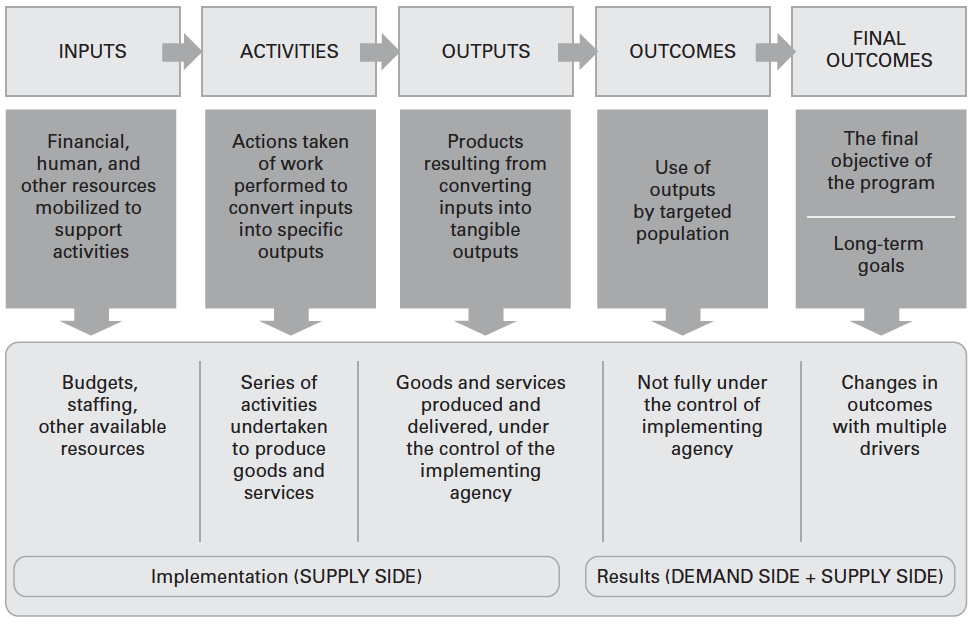
\includegraphics[keepaspectratio]{figures/results_chain}}
\caption{Results chain}
\end{figure}
\end{frame}

\begin{frame}{Results chain - example}
\phantomsection\label{results-chain---example}
\begin{itemize}
\tightlist
\item
  Government agency provides training about settlement to immigrants

  \begin{itemize}
  \tightlist
  \item
    \textbf{Inputs}: Staff from government agency, trainers, facilities,
    government budget, contact information of immigrants\\
  \item
    \textbf{Activities}: Design curriculum of training, select and
    prepare trainers, design, prepare, and distribute written material\\
  \item
    \textbf{Outputs}: Number of immigrants trained, number of written
    materials provided\\
  \item
    \textbf{Outcomes}: Immigrants behave differently based on
    information provided\\
  \item
    \textbf{Final outcomes}: Immigrants are (economically) more
    successful, higher well-being, less welfare spending for immigrants,
    reduced social tensions
  \end{itemize}
\end{itemize}
\end{frame}

\begin{frame}{Performance indicators (Outcomes)}
\phantomsection\label{performance-indicators-outcomes}
\begin{itemize}
\tightlist
\item
  Ideally use indicators along the whole results chain

  \begin{itemize}
  \tightlist
  \item
    Not only final outcomes\\
  \item
    Understand mechanisms\\
  \item
    Especially important if evaluation finds no effect on final
    outcome\\
  \end{itemize}
\item
  Selection of indicators should involve stakeholders\\
\item
  SMART indicators

  \begin{itemize}
  \tightlist
  \item
    \textbf{Specific}: Translates required information into operational
    measure\\
  \item
    \textbf{Measurable}: Information can be measured and obtained\\
  \item
    \textbf{Attributable}: Indicator is linked to the policy's efforts\\
  \item
    \textbf{Realistic}: Information can be obtained timely, with
    reasonable frequency, at reasonable cost\\
  \item
    \textbf{Targeted}: To the objective population
  \end{itemize}
\end{itemize}
\end{frame}

\end{document}
